\documentclass[11pt]{article}
\usepackage[a4paper,margin=2.3cm]{geometry}
\usepackage{amsmath,amssymb,amsthm}
\usepackage{enumitem}
\usepackage{tikz}
\usepackage[most]{tcolorbox}
\usepackage{microtype}

\setlength{\parindent}{0pt}
\setlength{\parskip}{6pt}
\renewcommand{\arraystretch}{1.3}

\newcommand{\R}{\mathbb{R}}
\newcommand{\Q}{\mathbb{Q}}
\newcommand{\Pow}{\mathcal{P}}
\newcommand{\T}{\mathcal{T}}
\newcommand{\B}{\mathcal{B}}

\newtcolorbox{ans}[1][]{breakable,colback=green!5,colframe=green!45!black,
  fonttitle=\bfseries,title={#1},left=6pt,right=6pt,top=4pt,bottom=4pt}
\newtcolorbox{note}[1][]{breakable,colback=orange!7,colframe=orange!70!black,
  fonttitle=\bfseries,title={#1},left=6pt,right=6pt,top=4pt,bottom=4pt}

\title{\textbf{Topology -- Problem Set 1}\\[2pt]\large Corrected solutions to Questions 11--14}
\author{}
\date{}

\begin{document}
\maketitle
\vspace{-2.5em}

% =====================================================================
\section*{Question 11}
% =====================================================================
Let $X$ be an infinite set, $a\in X$, and
\[
\T_a=\Pow(X\setminus\{a\})\ \cup\ \{V\subseteq X : a\in V\text{ and }X\setminus V\text{ is finite}\}.
\]
Call the first family $\mathcal A$ (sets \emph{not} containing $a$; every subset of $X\setminus\{a\}$ is in it) and the second family $\mathcal C$ (sets containing $a$ with finite complement). Note that every member of $\T_a$ either does not contain $a$ (and is in $\mathcal A$) or contains $a$ (and then is in $\mathcal C$).

\textbf{Claim: $\T_a$ is a topology.}

\textbf{(T1) $\emptyset,X\in\T_a$.} $\emptyset\subseteq X\setminus\{a\}$, so $\emptyset\in\mathcal A$. Also $a\in X$ and $X\setminus X=\emptyset$ is finite, so $X\in\mathcal C$.

\textbf{(T2) Arbitrary unions.} Let $\{V_\lambda\}_{\lambda\in\Lambda}\subseteq\T_a$ and $V=\bigcup_\lambda V_\lambda$.
\begin{itemize}[nosep]
\item If no $V_\lambda$ contains $a$ (this includes $\Lambda=\emptyset$), then every $V_\lambda\subseteq X\setminus\{a\}$, so $V\subseteq X\setminus\{a\}$ and $V\in\mathcal A$.
\item If some $V_{\lambda_0}\ni a$, then $V_{\lambda_0}\in\mathcal C$, so $X\setminus V_{\lambda_0}$ is finite. Since $V_{\lambda_0}\subseteq V$ we get $X\setminus V\subseteq X\setminus V_{\lambda_0}$, hence $X\setminus V$ is finite; and $a\in V$. So $V\in\mathcal C$.
\end{itemize}

\textbf{(T3) Finite intersections.} By induction it suffices to treat $U,V\in\T_a$.
\begin{itemize}[nosep]
\item If $a\notin U$ or $a\notin V$, then $a\notin U\cap V$, i.e.\ $U\cap V\subseteq X\setminus\{a\}$, so $U\cap V\in\mathcal A$.
\item If $a\in U$ and $a\in V$, then $U,V\in\mathcal C$, so $X\setminus U$ and $X\setminus V$ are finite. Then $X\setminus(U\cap V)=(X\setminus U)\cup(X\setminus V)$ is finite, and $a\in U\cap V$. So $U\cap V\in\mathcal C$.
\end{itemize}
Hence $\T_a$ is a topology. $\blacksquare$

\begin{ans}[What happens if $X$ is finite?]
Every $V\subseteq X$ has finite complement (a subset of the finite set $X$). So any $V\ni a$ lies in $\mathcal C$, and any $V\not\ni a$ lies in $\mathcal A$. Therefore $\T_a=\Pow(X)$, the \textbf{discrete topology}.\\
(For infinite $X$ it is \emph{not} discrete: $\{a\}$ is not open, because $a\in\{a\}$ but $X\setminus\{a\}$ is infinite.)
\end{ans}

% =====================================================================
\section*{Question 12}
% =====================================================================

Let $X$ be an infinite set and let $a,b\in X$ be distinct points.
The collection in the question is
\[
\T=\Pow(X\setminus\{a,b\})\cup
\{V\subseteq X: a\in V\text{ or }b\in V
\text{ and }X\setminus V\text{ is finite}\}.
\]

We use the usual convention for logical connectives: ``and'' has
precedence over ``or''. Thus, the condition defining the second
family is interpreted as
\[
 a\in V\quad\text{or}\quad
 \bigl(b\in V\text{ and }X\setminus V\text{ is finite}\bigr).
\]

\begin{ans}[Answer]
The collection $\T$ is \textbf{not a topology} on $X$.
We show that it is not closed under finite intersections.
\end{ans}

\textbf{Counterexample.} Consider
\[
 U=\{a,b\},\qquad V=X\setminus\{a\}.
\]
We first verify that both sets belong to $\T$.

Since $a\in U$, the set $U$ belongs to the second family,
and hence $U\in\T$.

Next, $b\in V$ and
\[
 X\setminus V=\{a\},
\]
which is finite. Therefore $V\in\T$ as well.

However,
\[
\begin{aligned}
 U\cap V
 &=\{a,b\}\cap(X\setminus\{a\})\\
 &=\{b\}.
\end{aligned}
\]
We now show that $\{b\}\notin\T$.

First, $\{b\}\notin\Pow(X\setminus\{a,b\})$, because
$b\notin X\setminus\{a,b\}$. Also, $a\notin\{b\}$, while
\[
 X\setminus\{b\}
\]
is infinite, since $X$ is infinite. Thus $\{b\}$ does not satisfy
\[
 a\in W\quad\text{or}\quad
 \bigl(b\in W\text{ and }X\setminus W\text{ is finite}\bigr)
\]
either. Consequently, $\{b\}\notin\T$.

We have therefore found $U,V\in\T$ such that
\[
 U\cap V=\{b\}\notin\T.
\]
Hence $\T$ is not closed under finite intersections, and so
\[
 \boxed{\T\text{ is not a topology on }X.}
\]
\hfill $\square$

\begin{note}[Remark on the logical grouping]
If the intended condition had instead been
\[
 (a\in V\text{ or }b\in V)
 \text{ and }X\setminus V\text{ is finite},
\]
then it would define a different collection. The counterexample above
addresses the expression as printed, using the standard precedence of
``and'' over ``or''.
\end{note}

% =====================================================================
\section*{Question 13}
% =====================================================================
Let $\B_1,\B_2,\B_3$ be the open balls, open rectangles $(\alpha,\beta)\times(\gamma,\delta)$, and open triangles (interiors of non-degenerate triangles) in $\R^2$. Let $\T_E$ denote the Euclidean topology and $B(p,\varepsilon)$ the open ball of radius $\varepsilon$ about $p$.

Recall: $\B$ is a \textbf{basis} on $Y$ if (B1) every point of $Y$ lies in some member of $\B$, and (B2) if $y\in B\cap B'$ with $B,B'\in\B$, there is $B''\in\B$ with $y\in B''\subseteq B\cap B'$.

\subsection*{Two lemmas used for all three collections}
\textbf{Lemma A.} Every member of $\B_1,\B_2,\B_3$ is Euclidean-open.\\
\emph{Proof.} Balls are open. A rectangle is a product of open intervals, hence open. An open triangle is an intersection of three open half-planes, hence open. $\square$

\textbf{Lemma B.} For every $p\in\R^2$ and $\varepsilon>0$, each $\B_i$ has a member $B$ with $p\in B\subseteq B(p,\varepsilon)$.\\
\emph{Proof.} \emph{Balls:} $B(p,\varepsilon)$ itself. \emph{Rectangles:} for $p=(p_1,p_2)$ take $R=(p_1-\tfrac\varepsilon2,p_1+\tfrac\varepsilon2)\times(p_2-\tfrac\varepsilon2,p_2+\tfrac\varepsilon2)$. A point of $R$ is at distance $<\sqrt{(\varepsilon/2)^2+(\varepsilon/2)^2}=\tfrac{\varepsilon}{\sqrt2}<\varepsilon$ from $p$. \emph{Triangles:} take the open equilateral triangle with centroid $p$ and circumradius $\varepsilon/2$. It lies in the closed disc of radius $\varepsilon/2$ about $p$, hence in $B(p,\varepsilon)$, and contains its centroid $p$. $\square$

\subsection*{(i) Basis axioms}
\textbf{(B1)} Given $p$, Lemma B with $\varepsilon=1$ gives a member of $\B_i$ containing $p$.

\textbf{(B2)} Let $B,B'\in\B_i$ and $p\in B\cap B'$. By Lemma A, $B\cap B'$ is Euclidean-open, so there is $\varepsilon>0$ with $B(p,\varepsilon)\subseteq B\cap B'$. By Lemma B there is $B''\in\B_i$ with $p\in B''\subseteq B(p,\varepsilon)\subseteq B\cap B'$.

So $\B_1,\B_2,\B_3$ are bases. $\blacksquare$

\subsection*{(ii) The identity maps are continuous}
\textbf{Claim: $\T_i=\T_E$ for $i=1,2,3$.}
\begin{itemize}[nosep]
\item $\T_i\subseteq\T_E$: members of $\T_i$ are unions of members of $\B_i$, which are Euclidean-open (Lemma A).
\item $\T_E\subseteq\T_i$: let $G$ be Euclidean-open and $p\in G$. Pick $\varepsilon$ with $B(p,\varepsilon)\subseteq G$ and, by Lemma B, $B_p\in\B_i$ with $p\in B_p\subseteq B(p,\varepsilon)\subseteq G$. Then $G=\bigcup_{p\in G}B_p\in\T_i$.
\end{itemize}
Now let $f:(\R^2,\T_i)\to(\R^2,\T_j)$, $f(x)=x$. If $G\in\T_j$, then $f^{-1}(G)=G\in\T_j=\T_E=\T_i$. So $f$ is continuous for all $i,j\in\{1,2,3\}$. $\blacksquare$

\subsection*{(iii) Conclusion}
The identity $(\R^2,\T_i)\to(\R^2,\T_j)$ is continuous exactly when every $G\in\T_j$ is in $\T_i$, i.e.\ $\T_j\subseteq\T_i$. By (ii) this holds for all pairs $(i,j)$, in both directions, so $\T_i\subseteq\T_j$ and $\T_j\subseteq\T_i$. Hence
\[
\T_1=\T_2=\T_3\ (=\T_E).\qquad\blacksquare
\]

% =====================================================================
\section*{Question 14}
% =====================================================================
Topologies on $\R$:
$\T_f$ (finite complement), $\T_c$ (countable complement), $\T_{\rm std}$ (basis $(a,b)$), $\T_K$ (basis $(a,b)$ and $(a,b)\setminus K$, $K=\{1,\tfrac12,\tfrac13,\dots\}$), $\T_\ell$ (basis $[a,b)$), $\T_u$ (basis $(a,b]$), $\T_{\rm left}$ (basis $(-\infty,b)$), $\T_{\rm right}$ (basis $(a,\infty)$).

Here $\T_f=\{\emptyset\}\cup\{U:\R\setminus U\text{ finite}\}$ and $\T_c=\{\emptyset\}\cup\{U:\R\setminus U\text{ countable}\}$. Also $\T_{\rm left}=\{\emptyset,\R\}\cup\{(-\infty,b)\}$ (a union of left rays is a left ray or $\R$), and similarly $\T_{\rm right}=\{\emptyset,\R\}\cup\{(a,\infty)\}$.

\textbf{Convention.} $\T\subseteq\T'$ means $\T'$ is \emph{finer}. To show a set is not open in a topology generated by a basis, show that some point of it lies in no basis element contained in the set.

\subsection*{Part 1: Inclusions}

\textbf{1. $\T_f\subsetneq\T_c$.} A finite set is countable, so every nonempty $\T_f$-open set is in $\T_c$. Strict: $\R\setminus\Q\in\T_c$ (complement $\Q$ countable) but $\notin\T_f$ ($\Q$ infinite).

\textbf{2. $\T_f\subsetneq\T_{\rm std}$.} If $U=\R\setminus\{x_1<\dots<x_k\}$, then $U=(-\infty,x_1)\cup(x_1,x_2)\cup\dots\cup(x_k,\infty)$, a union of open intervals (a ray is a union of bounded intervals, e.g.\ $(-\infty,x_1)=\bigcup_n(x_1-n,x_1)$). Strict: $(0,1)\in\T_{\rm std}$ is nonempty with infinite complement, so $\notin\T_f$.

\textbf{3. $\T_{\rm left},\T_{\rm right}\subsetneq\T_{\rm std}$.} $(-\infty,b)=\bigcup_n(b-n,b)$ and $(a,\infty)=\bigcup_n(a,a+n)$ are standard-open. Strict: $(0,1)$ is neither $\emptyset$, $\R$, a left ray, nor a right ray, so it is open in neither ray topology.

\textbf{4. $\T_{\rm std}\subsetneq\T_K$.} Every $(a,b)$ is a basis element of $\T_K$. Strict: $(-1,1)\setminus K\in\T_K$ contains $0$, but no interval $(-\delta,\delta)$ lies in it (it contains $1/n$ for large $n$), so it is not standard-open.

\textbf{5. $\T_{\rm std}\subsetneq\T_\ell$ and $\T_{\rm std}\subsetneq\T_u$.}
\[
(a,b)=\bigcup_{x\in(a,b)}[x,b)=\bigcup_{x\in(a,b)}(a,x].
\]
Strict: $[0,1)\in\T_\ell$ is not standard-open (no interval around $0$ fits inside), and $(0,1]\in\T_u$ is not standard-open (no interval around $1$ fits inside).

\textbf{6. $\T_K\subsetneq\T_u$.} Every $(a,b)$ is standard-open, hence $\T_u$-open. Take $x\in(a,b)\setminus K$; we find a basis set $(c,x]$ with $x\in(c,x]\subseteq(a,b)\setminus K$:
\begin{itemize}[nosep]
\item if $x\le0$: take $c=a<x$; then $(a,x]\subseteq(a,b)$ contains no positive numbers, hence no point of $K$;
\item if $x>0$: let $k=\max\{1/n:1/n<x\}=1/n_0$ with $n_0$ the least integer $>1/x$, and $c=\max(a,k)<x$. Every element of $K$ that is $<x$ is $\le k\le c$, and $x\notin K$, so $(c,x]\cap K=\emptyset$ and $(c,x]\subseteq(a,b)\setminus K$.
\end{itemize}
Thus $(a,b)\setminus K$ is a union of members of $\mathcal B_4$, i.e.\ $\T_u$-open. Strict: $(0,1]\in\T_u$ but $\notin\T_K$: a $\T_K$ basis element containing $1$ cannot be of the form $(a,b)\setminus K$ (as $1\in K$), so it is an interval $(a,b)$ with $b>1$, which is not contained in $(0,1]$.

\textbf{7. Transitive consequences.} $\T_f\subsetneq\T_{\rm std}\subsetneq\T_K,\T_\ell,\T_u$, so $\T_f$ is strictly coarser than all of $\T_K,\T_\ell,\T_u$; likewise $\T_{\rm left},\T_{\rm right}$ are strictly coarser than $\T_K,\T_\ell,\T_u$, and $\T_{\rm std}\subsetneq\T_u$.

\subsection*{Part 2: Incomparable pairs (with witnesses)}

\begin{itemize}
\item \textbf{$\T_K$ and $\T_\ell$.} $(-1,1)\setminus K\in\T_K\setminus\T_\ell$: every $[0,\varepsilon)$ contains some $1/n$. $[0,1)\in\T_\ell\setminus\T_K$: every $\T_K$-basis element containing $0$ contains negative numbers.
\item \textbf{$\T_\ell$ and $\T_u$.} $[0,1)\in\T_\ell\setminus\T_u$ (every $(c,0]$ contains negatives); $(0,1]\in\T_u\setminus\T_\ell$ (every $[1,\varepsilon)$ contains numbers $>1$).
\item \textbf{$\T_{\rm left}$ and $\T_{\rm right}$.} $(-\infty,0)\in\T_{\rm left}\setminus\T_{\rm right}$ and $(0,\infty)\in\T_{\rm right}\setminus\T_{\rm left}$.
\item \textbf{$\T_f$ and each ray topology.} $(-\infty,0)\in\T_{\rm left}$ has infinite complement, so $\notin\T_f$; and $\R\setminus\{0\}\in\T_f$ is not a left ray nor $\R$, so $\notin\T_{\rm left}$. The same witnesses (with $(0,\infty)$) work for $\T_{\rm right}$.
\item \textbf{$\T_c$ and each of $\T_{\rm std},\T_K,\T_\ell,\T_u,\T_{\rm left},\T_{\rm right}$.}
 \begin{itemize}[nosep]
 \item $\R\setminus\Q\in\T_c$ is not open in any of the six: every nonempty open set of each contains a nonempty interval minus at most $K$ (or a half-open interval or a ray), hence contains rational numbers.
 \item Conversely $(0,1)\in\T_{\rm std}\subseteq\T_K,\T_\ell,\T_u$ is open in them but $\notin\T_c$ (its complement is uncountable); and $(-\infty,0)\in\T_{\rm left}$, $(0,\infty)\in\T_{\rm right}$ are not in $\T_c$ for the same reason.
 \end{itemize}
\end{itemize}

\subsection*{Comparison table}
Entry in row $R$, column $C$: $\subsetneq$ means $\T_R$ is strictly coarser than $\T_C$; $\supsetneq$ strictly finer; $\parallel$ incomparable.

\begin{center}
\small
\begin{tabular}{c|cccccccc}
 & $\T_f$ & $\T_c$ & $\T_{\rm std}$ & $\T_K$ & $\T_\ell$ & $\T_u$ & $\T_{\rm left}$ & $\T_{\rm right}$\\\hline
$\T_f$ & $=$ & $\subsetneq$ & $\subsetneq$ & $\subsetneq$ & $\subsetneq$ & $\subsetneq$ & $\parallel$ & $\parallel$\\
$\T_c$ & $\supsetneq$ & $=$ & $\parallel$ & $\parallel$ & $\parallel$ & $\parallel$ & $\parallel$ & $\parallel$\\
$\T_{\rm std}$ & $\supsetneq$ & $\parallel$ & $=$ & $\subsetneq$ & $\subsetneq$ & $\subsetneq$ & $\supsetneq$ & $\supsetneq$\\
$\T_K$ & $\supsetneq$ & $\parallel$ & $\supsetneq$ & $=$ & $\parallel$ & $\subsetneq$ & $\supsetneq$ & $\supsetneq$\\
$\T_\ell$ & $\supsetneq$ & $\parallel$ & $\supsetneq$ & $\parallel$ & $=$ & $\parallel$ & $\supsetneq$ & $\supsetneq$\\
$\T_u$ & $\supsetneq$ & $\parallel$ & $\supsetneq$ & $\supsetneq$ & $\parallel$ & $=$ & $\supsetneq$ & $\supsetneq$\\
$\T_{\rm left}$ & $\parallel$ & $\parallel$ & $\subsetneq$ & $\subsetneq$ & $\subsetneq$ & $\subsetneq$ & $=$ & $\parallel$\\
$\T_{\rm right}$ & $\parallel$ & $\parallel$ & $\subsetneq$ & $\subsetneq$ & $\subsetneq$ & $\subsetneq$ & $\parallel$ & $=$
\end{tabular}
\end{center}

\subsection*{Hasse diagram}
An arrow goes from the coarser topology to the finer one. Only the covering relations are drawn; all other strict inclusions follow by transitivity (e.g.\ $\T_f\subsetneq\T_K$, $\T_{\rm left}\subsetneq\T_\ell$), and any two topologies not joined by a directed path are incomparable.

\begin{center}
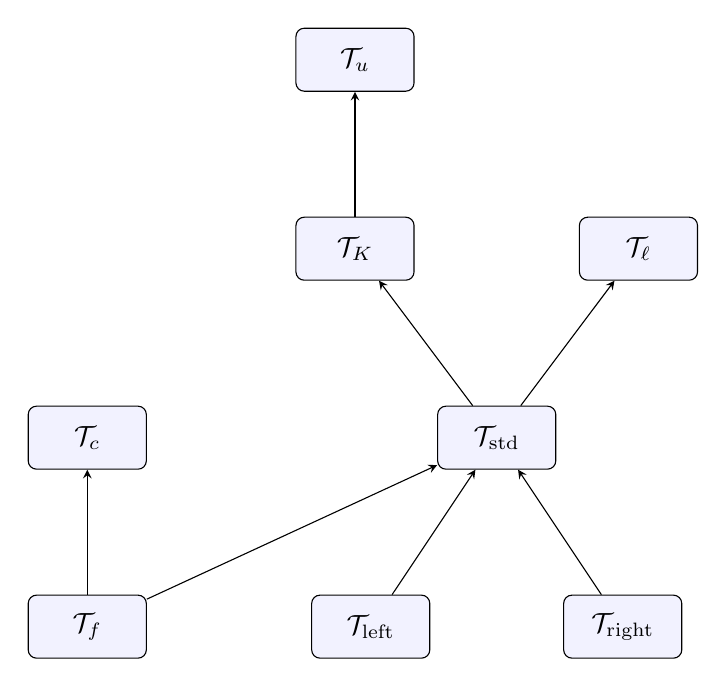
\begin{tikzpicture}[>=stealth,node distance=1cm,
  t/.style={draw,rounded corners=3pt,minimum width=1.5cm,minimum height=0.8cm,fill=blue!5}]
  \node[t] (f)  at (-5.2,0) {$\T_f$};
  \node[t] (c)  at (-5.2,2.4) {$\T_c$};
  \node[t] (le) at (-1.6,0) {$\T_{\rm left}$};
  \node[t] (ri) at (1.6,0) {$\T_{\rm right}$};
  \node[t] (st) at (0,2.4) {$\T_{\rm std}$};
  \node[t] (k)  at (-1.8,4.8) {$\T_K$};
  \node[t] (l)  at (1.8,4.8) {$\T_\ell$};
  \node[t] (u)  at (-1.8,7.2) {$\T_u$};
  \draw[->] (f) -- (c);
  \draw[->] (f) -- (st);
  \draw[->] (le) -- (st);
  \draw[->] (ri) -- (st);
  \draw[->] (st) -- (k);
  \draw[->] (st) -- (l);
  \draw[->] (k) -- (u);
\end{tikzpicture}
\end{center}

\begin{ans}[Final summary]
Strict chains: $\T_f\subsetneq\T_c$; $\ \T_f,\T_{\rm left},\T_{\rm right}\subsetneq\T_{\rm std}$; $\ \T_{\rm std}\subsetneq\T_K\subsetneq\T_u$; $\ \T_{\rm std}\subsetneq\T_\ell$.\\
Incomparable: $\T_K\parallel\T_\ell$, $\T_\ell\parallel\T_u$, $\T_{\rm left}\parallel\T_{\rm right}$, $\T_f\parallel\T_{\rm left},\T_{\rm right}$, and $\T_c$ is comparable only with $\T_f$ (where $\T_f\subsetneq\T_c$).
\end{ans}

\end{document}
